\documentclass{standalone}
\usepackage{tikz}
\usepackage{ctex,siunitx}
\setCJKmainfont{Noto Serif CJK SC}
\usepackage{tkz-euclide}
\usepackage{amsmath}
\usetikzlibrary{patterns, calc}
\usetikzlibrary {decorations.pathmorphing, decorations.pathreplacing, decorations.shapes,}
\begin{document}
\small
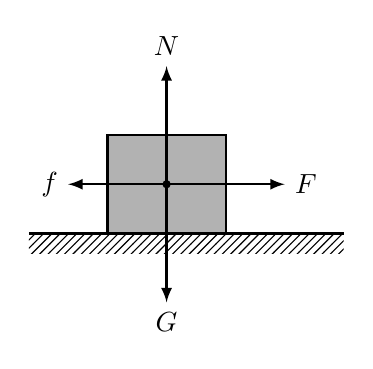
\begin{tikzpicture}[>=latex, thick,scale=1]
  % \useasboundingbox(-1,-0.75)rectangle(3.7,1.4);
  \fill [fill=black!30, draw] (2,0) rectangle (3.5,1.25);
  \fill [pattern = north east lines] (1,-.25) rectangle (5,0);
  \draw (1,0)--(5,0);
  \draw[->] (5.5/2,1.25/2)--(5.5/2, 1.25/2+1.5) node[above]{$N$};
  \draw[->] (5.5/2,1.25/2)--(5.5/2, 1.25/2-1.5) node[below]{$G$};
  \draw[->] (5.5/2,1.25/2)--(5.5/2-1.25, 1.25/2)node[left]{$f$};
  \draw[->] (5.5/2,1.25/2)--(5.5/2+1.5, 1.25/2) node[right]{$F$};
  % \node at (5.5/2, 1.25/2+1.75) {$N$};
  % \node at (5.5/2, 1.25/2-1.75) {$G$};
  % \node at (5.5/2-1.5, 1.25/2) {$f$};
  % \node at (5.5/2+2.75, 1.25/2) {$F$};
  \fill (5.5/2,1.25/2) circle[radius=1.5pt];
  % \fill (5.5/2,1.25/2) circle[radius=1.5pt];
\end{tikzpicture}
\end{document}